%%%%%%%%%%%%%%%%%%%%%%%%%%%%%%%%%%%%%%%%%%%%%%%
% BEGIN ROTATIES EN IMPULSMOMENT
%%%%%%%%%%%%%%%%%%%%%%%%%%%%%%%%%%%%%%%%%%%%%%%

\newcommand{\bra}[1]{\langle #1 \vert}
\newcommand{\ket}[1]{\vert #1 \rangle}
\newcommand{\bm}[1]{\mbox{\boldmath $#1$}}
\newcommand{\be}{\begin{equation}}
\def\lambdabar{\rlap{$^-$} \lambda}
\newcommand{\ee}{\end{equation}}
\newcommand{\bea}{\begin{eqnarray}}
\newcommand{\eea}{\end{eqnarray}}
\newcommand{\bean}{\begin{eqnarray*}}
\newcommand{\eean}{\end{eqnarray*}}


\chapter{Rotaties en impulsmoment}

In dit hoofdstuk bekijken we fysica van rotatie van objecten. Daarvoor introduceren we de begrippen krachtmoment, traagheidsmoment, impulsmoment (en het behoud daarvan) en energie in rotatie. We zullen dit alles ook in vector vorm bestuderen, zodat we bijvoorbeeld de precessie van een tol of gyroscoop kunnen begrijpen. Niet alles wordt hier behandeld (is nog in ontwikkeling), dus bestudeer vooral ook de bijbehorende hoofdstukken uit Giancoli.
\newline
\newline
Stof uit Giancoli:
\begin{itemize}
\item Hoofdstuk 10 en 11
\end{itemize}



\section{Kinetische energie van roterend systeem en traagheidsmoment
\label{kinrot}}

Rotaties in drie dimensies worden gekenmerkt door een rotatie\-as. 
De beweging ten gevolge van die rotatie vindt plaats in vlakken
die loodrecht op die as staan. We herhalen even de kenmerkende
begrippen voor de beweging in het rotatie\-vlak, waarbij we het
snijpunt met de rotatie\-as als oorsprong kiezen en werken met
afstand $b$ en hoek $\varphi$:
\\[0.2cm]
\begin{minipage}{6.5cm}
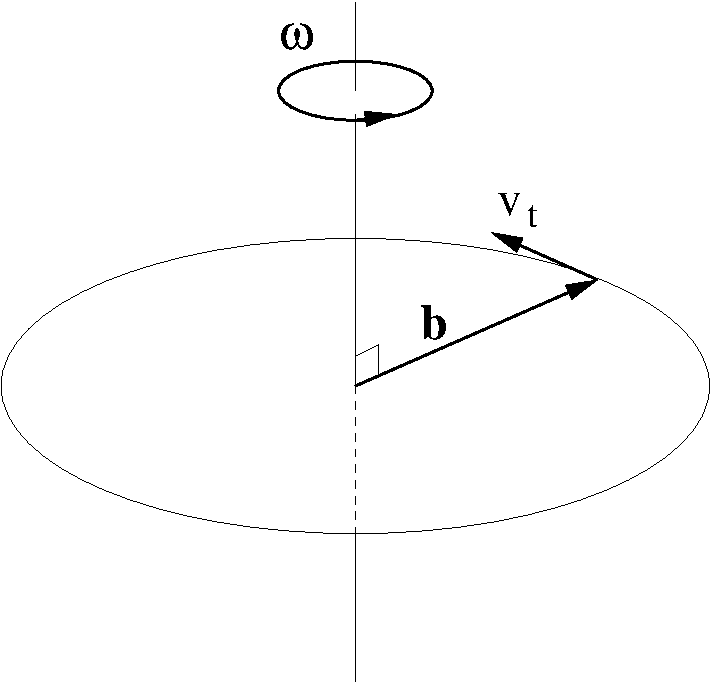
\epsfig{file=Traagheidrotatie.pdf, width=5.5cm}
\end{minipage}
\begin{minipage}{9cm}
\bean
\mbox{hoeksnelheid:} &&\omega = \dot{\varphi},
\\
\mbox{hoekversnelling:} &&\alpha = \dot{\omega} = \ddot{\varphi},
\\
\mbox{tangenti\"ele snelheid:} &&v_{\rm t} = \omega\,b,
\\
\mbox{tangenti\"ele versnelling:} &&a_{\rm t} = \alpha\,b,
\\
\mbox{centripetale versnelling:} &&a_{\rm c} = \omega^2\,b 
= v_{\rm t}^2/b,
%\\
%\mbox{traagheidsmoment:} && I = mb^2,
%\\
%\mbox{krachtmoment:} && \tau = F_t\,b = m\,a_t\,b = mb^2\,\alpha = I\,\alpha.
\eean
\end{minipage}
\\[0.2cm]
Om een uitdrukking voor de kinetische energie van een roterend systeem 
te vinden gaan we uit van een vaste rotatie\-as. We zien dat de kinetische
energie gelijk is aan
\be
K = \tfrac{1}{2}\sum_i m_i\,\bm v_i^2 =
\tfrac{1}{2}\sum_i m_i\,\bm b_i^2\,\omega^2   
= \tfrac{1}{2}\,I\,\omega^2,
\ee
waar $\bm b_i$ de positie vector in het rotatievlak is met als lengte de 
afstand van de massa $m_i$ tot de as; 
dus als we rotaties om de $z$-as bekijken dan is $b_i^2 = x_i^2+y_i^2$.
De grootheid $I$ heet het {\em traagheidsmoment} (Engels: moment of inertia)
rond de rotatie\-as,
\be
I = \sum_i m_i\,b_i^2,
\ee
Voor een uitgebreid systeem met massaverdeling $\rho(\bm r)$ wordt dit  
\be
I = \int d^3r\ (x^2+y^2)\,\rho(x,y,z) 
= \int dz\,b^3\,db\,d\varphi\,\rho(b,\varphi,z).
\ee
We merken op dat het traagheidsmoment afhangt van de rotatie\-as
Voorbeelden van traagheidsmomenten zijn:
\bea
\mbox{homogene bol (straal $R$, as door middelpunt):} && I = \tfrac{2}{5}\,MR^2,
\\
\mbox{holle bol (straal $R$, as door middelpunt):} && I = \tfrac{2}{3}\,MR^2,
\\
\mbox{staaf (lengte $L$, as door middelpunt loodrecht op staaf):} && 
I = \tfrac{1}{12}\,ML^2,
\\
\mbox{staaf (lengte $L$, as door eindpunt loodrecht op staaf):} && 
I = \tfrac{1}{3}\,ML^2,
\eea
Het traagheidsmoment t.o.v.\ een as door het zwaartepunt wordt meestal 
bedoeld als we praten over {\em het} traagheidsmoment van een object. 
Er zijn dan natuurlijk nog meerdere
traagheidsmomenten afhankelijk van de richting van die as.
Uitgaande van een van die assen door het zwaartepunt kunnen we voor
alle assen parallel daaraan op afstand $h$ het traagheidsmoment vinden
via 
\bea
I_h = \sum_i m_i\,(\bm b_i + \bm h)^2 & = &
\sum_i m_i\,\bm b_i^2 + \bm h\cdot \left(\sum_i m_i\,\bm b_i\right) 
+\bm h^2\,\sum_i m_i 
\nonumber \\& = &
I_{\rm cm} + M\,h^2,
\eea
waar de tweede term in de laatste uitdrukking in eerste regel nul is omdat
de $\bm b_i$ gewogen met massa's $m_i$ juist het zwaartepunt in het 
rotatievlak geven, wat we als oorsprong hadden genomen.

Gecombineerd met een beweging van het zwaartepunt vinden we voor de
kinetische energie van een eenparig bewegend roterend object op 
dezelfde wijze,
\be
K = \tfrac{1}{2}\sum_i m_i
\,\left(\bm V+ \bm v_i\right)^2 =
\tfrac{1}{2}\,M\bm V^2 + \tfrac{1}{2}\,I_{\rm cm}\,\omega^2.
\label{kinrot-1}
\ee

\section{Krachtmoment en behoud van impulsmoment}

We beginnen weer met de rotatie die zich in een vlak afspeelt.
We hebben al eerder gezien dat een cirkelbeweging altijd een versnelde
beweging is met een naar het middelpunt van de cirkel gerichte
versnelling $a_c$. Er is dus altijd een radi\"ele kracht nodig
(bv.\ spankracht of gravitatiekracht) om een object in een 
cirkelbaan te houden. De grootte van de (naar het centrum gerichte) 
centripetale kracht is 
\be
F_c = m\,a_c = m\,\omega^2\,b = \frac{m\,v_t^2}{b}.
\ee
Er kan ook nog een kracht langs de baan zijn die dan de tangenti\"ele
versnelling oplevert,
\[
F_t = m\,a_t = mb\,\alpha = mb\,\frac{d\omega}{dt}.
\]
%
\\[0.4cm]
%\noindent
\fbox{
\begin{minipage}{15.5cm}
{\bf Uitproduct van vectoren}
\\[0.2cm]
Rotaties worden gekenmerkt door een rotatievlak. Zo'n vlak wordt in drie
dimensies ook vastgelegd wanneer we de vector loodrecht op het vlak geven.
In drie dimensies wordt daarbij veelvuldig gebruik gemaakt van het 
{\em uitproduct} (Engels: vector product) van vectoren.
% \\[0.2cm]
\begin{minipage}{7.5cm}
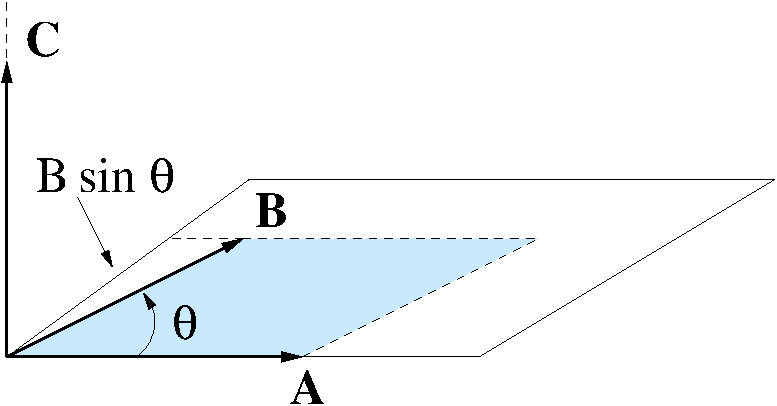
\epsfig{file=Outerproduct.pdf,width=7cm}
\end{minipage}
\begin{minipage}{8cm}
Het uitproduct van twee vectoren $\bm A$ en $\bm B$,
\be
\bm C = \bm A \times \bm B,
\ee
is een vector $\bm C$ die loodrecht op $\bm A$ en $\bm B$ staat (en dus
ook op het vlak waarin $\bm A$ en $\bm B$ liggen). 
De richting t.o.v.\ het vlak wordt bepaald met de kurketrekker\-regel.
De lengte van de vector is 
\be
\vert \bm C\vert = \vert \bm A\vert\,\vert \bm B\vert \,\sin\theta ,
\ee
\end{minipage}
\\[0.4cm]
waar $\theta$ de hoek tussen $\bm A$ en $\bm B$ is.
We merken op dat $\vert \bm B\vert\,\sin\theta$ precies de grootte
van de projectie op de richting loodrecht op $\bm A$ is.
De grootte van het uitproduct is dus precies het oppervlak van het
parallellogram opgespannen door $\bm A$ en $\bm B$ of tweemaal het
oppervlak van de driehoek waarvan $\bm A$ en $\bm B$ de zijden vormen.
Het uitproduct heeft een aantal eigenschappen zoals
\bea
&&
\bm A \times \bm B = -\bm B\times \bm A,
\\&&
\bm A \times \bm A = 0,
\\&&
\bm A \times (\bm B + \bm C) = \bm A \times \bm B + \bm A\times\bm C,
\\&&
\bm A\cdot (\bm B \times \bm C) = 
\bm B\cdot (\bm C \times \bm A) = 
\bm C\cdot (\bm A \times \bm B), 
\\&&
\bm A \times (\bm B \times \bm C) =
(\bm A\cdot \bm B)\,\bm C - (\bm A\cdot \bm C)\,\bm B ,
\\&&
\frac{d}{dt}\left(\bm A \times \bm B\right)
= \left( \frac{d\bm A}{dt}\times\bm B\right)
+ \left( \bm A \times \frac{d\bm B}{dt}\right).
\eea
Uitdrukkingen gebruikmakend van co\"ordinaten kunnen we gemakkelijk vinden
door gebruik te maken van de lineariteit van het uitproduct, de expansie
$\bm A = A_x\,\hat{\bm x} + A_y\,\hat{\bm y} + A_z\,\hat{\bm z}$ en de
basis\-eigenschappen $\hat{\bm x} \times \hat{\bm y} = \hat{\bm z}$, 
etc.\ (cyclisch verwisselen). Voor $\bm C = \bm A\times \bm B$ vinden 
we
\be
C_x = A_y\,B_z - A_z\,B_y, \quad
C_y = A_z\,B_x - A_x\,B_z, \quad
C_z = A_x\,B_y - A_y\,B_x. 
\ee
\end{minipage}
}
\\[0.5cm]
Hieruit zien we dat de hoekversnelling tengevolge van de tangenti\"ele
kracht gegeven wordt door
\be
\alpha = \frac{F_t}{m\,b} = \frac{b\,F_t}{I} = \frac{\tau}{I} 
\qquad \mbox{of} \qquad  \tau = I\,\alpha.
\label{torque}
\ee
De grootheid $\tau = b\,F_t$ heeft een speciale naam, het illustreert hoe
een hoekversnelling bij een object met een traagheidsmoment $I$
bepaald wordt door {\em arm}$\times${\em kracht}, bekend als het
krachtmoment (Engels: torque). Vergelijking~\ref{torque} is de analogie
van Newton in het geval van rotaties.

Welke arbeid verrichten deze krachten?. De centripetale kracht staat 
loodrecht op de verplaatsing, dus verricht bij een cirkelbaan
geen arbeid\footnote{
Arbeid wordt er wel verricht als de massa naar binnen of buiten
wordt bewogen.}. 
Een tangenti\"ele kracht verricht wel arbeid, welke precies ten goede
komt aan de in de vorige paragraaf berekende kinetische energie. 
In een tijd $dt$ is de verplaatsing gelijk aan $b\,d\phi$ = $b\,\omega dt$
\be
dW = F_t\,b\,d\phi = \tau\,d\phi = \tau\,\omega\,dt
\ee
Dit kunnen we herschrijven als
\[
\tau\,\omega = I\,\frac{d\omega}{dt}\,\omega 
= \frac{d}{dt}\left(\frac{1}{2}\,I\omega^2\right),
\]
waaruit we zien dat arbeid ten goede komt aan de kinetische energie van
het roterende object.

Het krachtmoment kunnen we algemener behandelen als vectorgrootheid.
We hebben behoud van energie en impuls gevonden door te zoeken
naar grootheden die veranderen als er krachten worden uitgeoefend
op een object, om precies te zijn in hoofdstuk~\ref{energie-impuls}
hebben we gekeken naar $\bm F\cdot \bm v$ en in hoofstuk~\ref{impuls}
naar $\bm F$ zelf.
Voor rotaties beschouwen we de kracht\-component loodrecht op $\bm r$
waarvoor we het uitproduct gebruiken,
\be
\bm r \times \bm F = m\,\left(\bm r \times \frac{d\bm v}{dt}\right)
= m\,\frac{d}{dt}\left(\bm r \times \bm v\right)
= \frac{d\bm \ell}{dt},
\ee
waar het {\em impulsmoment} (Engels: angular momentum) gegeven wordt door
\be
\bm \ell = \bm r \times \bm p = m\,\bm r\times \bm v.
\ee
De linkerkant staat bekend als het {\em krachtmoment} (Engels: torque) 
$\bm \tau = \bm r \times \bm F$, nu netjes als vectorgrootheid.

Voor een voorwerp bestaande uit componenten, krijgen we
\bea
&&
\bm L = \sum_i \bm \ell_i = \sum_i \bm r_i\times \bm p_i,
\\&&
\bm \tau_{\rm net} = \sum_i \bm r_i \times \bm F_i = \frac{d\bm L}{dt},
\label{newtonrotatie}
\eea
d.w.z.\ voor het gecombineerde systeem hebben we {\em behoud van
totaal impulsmoment} $\bm L$ als het netto krachtmoment nul is. 
Dit is bijvoorbeeld het geval als er alleen onderlinge krachten zijn,
bijvoorbeeld het zonne\-stelsel of een vrij bewegend atoom of molecuul.
We merken op dat in principe bovenstaande uitdrukkingen afhangen van
de keuze van de oorsprong, maar dat geldt voor linkerkant {\em en} 
rechterkant van de vergelijkingen.

Het ontbreken van krachtmoment en behoud van impulsmoment heeft een
fundamentele relatie met rotatie\-symmetrie. 
Bijvoorbeeld de Aarde bevindt zich in het
zwaartekrachtveld van de Zon. Maar de kracht is langs de Aarde-Zon lijn
gericht. Dus met de Zon als oorsprong (of t.o.v.\ het zwaartepunt Aarde-Zon)
zien we dat het krachtmoment nul is (uitproduct van parallelle vectoren) 
en het impulsmoment van het systeem Aarde-Zon is dus behouden. 
We kunnen ook kijken naar de 
potentiaal\-functie, waarvan de kracht is afgeleid 
(de kracht is de gradient van de potentiaal). Dat is in rotatie-symmetrische situaties
een {\em centrale potentiaal}, $U(\bm r) = U_c(r)$, 
die alleen afhangt van de grootte van de onderlinge afstand. De kracht
\be
\bm F = -\bm \nabla U_c(r) = -\frac{1}{r}\,\frac{dU_c}{dr}\,\hat{\bm r}.
\label{krachtpot}
\ee
is dan radi\"eel en het bijbehorende krachtmoment is nul.
\\[0.2cm]
\fbox{\begin{minipage}{15.5cm}
Dit illustreert het fundamentele verband tussen {\em rotatie\-symmetrie} 
en {\em behoud van impulsmoment}.
\end{minipage}
}

\section{Rotatiesnelheid en impulsmoment als vectorgrootheid}

We kijken naar de snelheden van een star (samenhangend)
roterend systeem. T.o.v.\ een oorsprong ergens op de rotatie\-as
hebben we 
\be
\bm v_i = \bm\omega \times \bm r_i,
\ee
waar $\bm\omega$ een vector is met de hoeksnelheid $\omega$ als lengte en
de rotatie-as als richting (met positief/negatief bepaald via de 
kurke\-trekker\-regel).
Het is eenvoudig na te gaan dat de grootte van de snelheid gevonden wordt
als het product van $\omega$ en de afstand $b_i$ tot de as en de 
tangenti\"ele richting staat loodrecht op de rotatie\-as en $\bm r_i$. 
De algemene uitdrukking voor het impulsmoment van het hele systeem is
\be
\bm L = \sum_i m_i\,\bm r_i\times \bm v_i
= \sum_i m_i\,\bm r_i\times (\bm \omega \times \bm r_i)
= \sum_i m_i 
\left(\bm r_i^2\,\bm \omega - (\bm\omega\cdot \bm r_i)\bm r_i\right).
\label{momentgeneral}
\ee
Expliciet in componenten hebben we
\[
\bm\omega = \left\lgroup \begin{array}{c}
0 \\ 0 \\ \omega \end{array}\right\rgroup,
\quad
\bm r_i = \left\lgroup \begin{array}{c}
x_i \\ y_i \\ z_i \end{array}\right\rgroup,
\quad
\bm\omega\times\bm r_i = \left\lgroup \begin{array}{c}
-\omega\,y_i \\ \omega\,x_i \\ 0 \end{array}\right\rgroup,
\quad
\bm r_i\times\left(\bm\omega\times\bm r_i\right) 
= \left\lgroup \begin{array}{c}
-\omega\,x_i\,z_i \\ -\omega\,y_i\,z_i \\ \omega(x_i^2+y_i^2) 
\end{array}\right\rgroup.
\]
Als het systeem symmetrisch is om de z-as is er voor iedere positieve
$x_i$ een $-x_i$ bijdrage in de som en idem voor $y_i$, dus de eerste
twee componenten zullen na sommatie nul geven. We hebben dan
\be
\bm L = I\,\bm \omega,
\ee
waar $I$ het in paragraaf~\ref{kinrot} besproken traagheidsmoment is.
Het resultaat laat zien dat voor een mooi symmetrisch systeem
behoud van impuls kan corresponderen met een uniform roterend 
systeem. 
Voor een niet-symmetrisch systeem moeten we terug 
naar vgl.~\ref{momentgeneral}, 
de situatie is ingewikkelder en de rotatie\-as van
systeem zal in het algemeen precessies uitvoeren t.o.v.\ een
vaste as in de ruimte. 
Gebruikmakend van de uitdrukking voor kinetische energie in 
vgl.\ \ref{kinrot} van een
roterend systeem zien we dat uitgedrukt in termen van het impulsmoment
\be
K = \frac{1}{2}\,I\,\bm \omega^2 = \frac{\bm L^2}{2I}.
\ee
(Vergelijk met $K = \tfrac{1}{2}M\bm V^2 = \bm P^2/2M$.)
Verder kunnen we vergelijking~\ref{newtonrotatie} schrijven als
\be
\bm\tau_{\rm net} = \frac{d\bm L}{dt} = I\,\dot{\bm \omega} = I\,\bm\alpha.
\label{newtonrotatie-2}
\ee
(Vergelijk met $\bm F_{\rm net} = d\bm P/dt = M\,\bm A$.)

Om het impulsmoment t.o.v.\ een willekeurig punt te bepalen is het
nuttig om de zwaartepunt-co\"ordinaat af te splitsen,
$\bm r_i = \bm R + \bm r_{{\rm cm}\,i}$ en idem voor $\bm v_i$. Omdat 
$\sum_i m_i\bm r_{{\rm cm}\,i} = 0$, vinden we
\be
\bm L = \bm R \times M\bm V
+ \sum_i \bm r_{{\rm cm}\,i} \times m_i\,\bm v_{{\rm cm}\,i}
= \bm L_{\rm baan} + \bm L_{\rm spin}.
\ee
Het impulsmoment $\bm L_{\rm spin}$ (ook kortweg spin $\bm S$ genoemd)
is onafhankelijk van de keuze van oorsprong. Voor een uit twee objecten
bestaand systeem is het eenvoudig om te zien dat
\be
\bm L_{\rm spin} = \bm r\times \mu\,\bm v,
\ee
waar $\bm r$ en $\bm v$ de relatieve co\"ordinaten zijn 
(ten opzichte van het massamiddelpunt).

\section{*Impulsmoment en quantummechanica}

Dit gedeelte behoort niet tot de stof, maar geeft alvast een 'sneak preview' op wat er later komen gaat. Tot nu toe hebben we impulsmoment behandeld als klassieke grootheid. Maar klassieke 
mechanica werkt niet meer bij de allerkleinste schalen, zoals in atomen. Ook in atomen is er impulsmoment, bijvoorbeeld van de electronen. Maar op atomaire schaal moeten we impulsmoment quantummechanisch behandelen. De eenheid van impuls\-moment
(kg\,m$^2$/s = J\,s) is ook de eenheid voor de constante van Planck.
We kunnen een impulsmoment dus in principe als een veelvoud van
de constante van Planck beschouwen.

Kijken we eerst naar het impulsmoment langs een bepaalde richting
(we kiezen voor gemak z-richting), dan blijkt
quantummechanisch baan\-impuls\-moment alleen als heeltallige
veelvouden van $\hbar = h/2\pi$ voor te komen,
\[
\ell_z = m_\ell\,\hbar \quad\mbox{met}\quad m_\ell \ \mbox{heeltallig}.
\]
Op het meest elementaire niveau blijken deeltjes ook als half\-tallige
veelvouden voor te komen, 
\[
s_z = m_s\,\hbar \quad\mbox{met}\ m_s \ \mbox{halftallig \'of heeltallig}.
\]
bijvoorbeeld de spin van een elektron
of een quark kunnen een spin $s_z = \pm \hbar/2$ (de verschillen
kunnen alleen heeltallig zijn). 

Verder blijken impuls\-momenten altijd te precederen, wat ook betekent
dat de spin niet strikt langs een as kan liggen. Quantum\-mechanisch
blijkt de lengte van baan\-impulsmomenten gegeven te worden
door 
\[
\bm \ell^2 = \ell(\ell + 1)\,\hbar^2 \quad \mbox{met} 
\quad \ell = 0, 1, 2, \ldots
\]
waarbij de maximale en minimale waarden toegestaan voor $\ell_z$ 
de waarden $m_\ell = \pm\ell$ zijn en alle heeltallige tussen\-liggende 
waarden toegestaan zijn. Op dezelfde manier hebben we voor spin
\[
\bm s^2 = s(s + 1)\,\hbar^2 \quad \mbox{met} 
\quad s = 0, 1/2, 1, 3/2, \ldots
\]
weer met voor $s_z$ maximale en minimale waarden $m_s = \pm s$ en
(in heeltallige stappen) toegestane tussenliggende waarden.

\section{Wat moet ik weten en kunnen?}

Na dit hoofdstuk moet je weten:
\begin{itemize}
\item Wat impulsmoment ($L$) is en waarom en onder wat voor omstandigheden impulsmoment een behouden grootheid is.
\item Wat een krachtmoment ($\tau$) is en hoe dit rotatie beinvloed.
\item Hoe impultmoment en krachtmoment in vectorvorm werkt.
\item Wat het traagheidmoment ($I$) is, en hoe dit bepaald kan worden.
\item Wat de energie in rotatie is.
\item Wat precessie is (zie Giancoli) en het Coriolis effect.
\end{itemize}
En je moet kunnen:
\begin{itemize}
\item Uitrekenen van impulsmoment, krachtmoment, traagheidmoment, energie in rotatie, en precessie snelheid.
\item Bepalen of impulsmoment behouden is of niet, en kunnen werken met het vectormodel van krachtmoment en impulsmoment (zoals gebruik van het uitproduct).
\end{itemize}

\section{Opgaven}

\begin{enumerate}
\item Giancoli hoofdstuk~9. {\bf Problems}: 13,25,47,50,56,66,77,41,69
\item Giancoli hoofdstuk~10. {\bf Problems}: 8,15,22,30,38,47,58,75,51,68

\end{enumerate}
%%%%%%%%%%%%%%%%%%%%%%%%%%%%%%%%%%%%%%%%%%%%%%%
% EINDE ROTATIES EN IMPULSMOMENT
%%%%%%%%%%%%%%%%%%%%%%%%%%%%%%%%%%%%%%%%%%%%%%%


